\subsection{Field study}

The customer for this project, Artsdatabanken, also known as the Norwegian Biodiversity Information Center, is devoted to providing public biodiversity information. It keeps species records of birds, insects, and plants among other things. It currently has 6 million registered species, 85\% of which birds\cite{arts:field-study}. \newline

Species are registered individually or in collaboration and in company of two or more individual obervers. Observations / Sightings are a collection of species and attributes about the species such as name, the number of observed individuals, the activity they were engaged in during observation, age, sex, observation start/end with date and time, observer, co-observer, and location. Registered data quality is validated by reputation and bibliometric qualities.

\begin{figure}[htb]
	\centering
	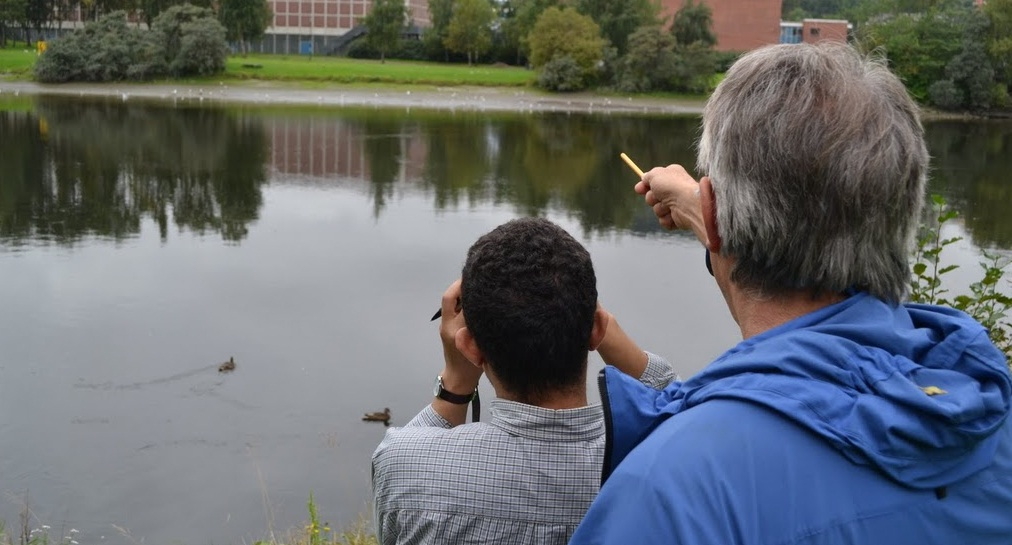
\includegraphics[width=0.8\textwidth]{prestudy/field_study/field_stud.jpg}
	\caption{Counting number of different species}
	\label{fig:field_study}
\end{figure}

Sighting location and species picture are non-negotiable features of the system. Location can be known and already registered or can be conjured up using GPS coordinates. Locations are classified as super and sublocations. Pictures are used based on convenience such as for plants and immobile species candidates.

The customer wants the team to provide full mobility to the observers with offline data storage and synchronization, and also a full comparison of the iOS and Android platform possibilities, and what they stand to gain or lose in adopting the technologies. The customer also suggested keeping all the functionalities of the desktop, and breaking down those functionalities on the mobile device.

During any sighting, the recommendation is to use approximate number of species seen for common species, while being strictly accurate for rare species or not mentioning a number. Each observation is limited to one type of species, for example birds, plants or mammals.

\begin{figure}[htb]
	\centering
	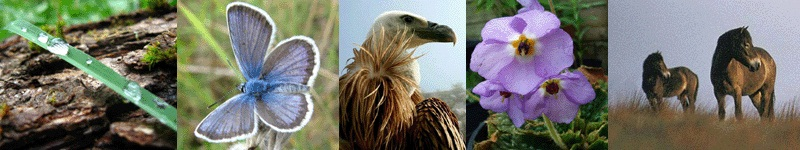
\includegraphics[width=1\textwidth]{prestudy/field_study/flora_fauna_Nikola.jpg}
	\caption{Observation can include rare and endangered species}
	\label{fig:field_study_species}
\end{figure}


